% ============================================================
% CHAPTER 7: EXPERIMENTS AND RESULTS
% ============================================================
\chapter{Experiments and Results}

\section{Experimental Setup}

\paperref{Section 4 - Experiment}

\subsection{Training Configuration}

\begin{table}[H]
\centering
\caption{Training Hyperparameters từ Paper}
\begin{tabular}{lccccc}
\toprule
\textbf{Parameter} & \textbf{CNN} & \textbf{ResNet} & \textbf{ViT-v1} & \textbf{ViT-v2} & \textbf{ViT-ResNet} \\
\midrule
Learning Rate & 0.001 & 0.001 & 0.001 & 0.0001 & 0.0001 \\
Batch Size & 32 & 32 & 32 & 64 & 64 \\
Epochs & 30 & 30 & 30 & 60 & 60 \\
Optimizer & Adam & Adam & Adam & Adam & Adam \\
\bottomrule
\end{tabular}
\end{table}

\subsection{Hardware Setup}

\begin{tcolorbox}[colback=blue!5!white,colframe=blue!75!black,title=Training Environment]
\textbf{Paper Environment:}
\begin{itemize}
    \item Platform: Google Colab
    \item GPU: NVIDIA T4 / A100
    \item Framework: TensorFlow 2.x / Keras
\end{itemize}

\textbf{Our PyTorch Implementation:}
\begin{itemize}
    \item Platform: Local / Google Colab
    \item GPU: NVIDIA GPU với CUDA
    \item Framework: PyTorch 2.x
\end{itemize}
\end{tcolorbox}

\section{Evaluation Metrics}

\subsection{Accuracy}

\begin{equation}
\text{Accuracy} = \frac{\text{Correct Predictions}}{\text{Total Predictions}}
\end{equation}

\begin{tcolorbox}[colback=orange!5!white,colframe=orange!75!black,title=Cảnh báo: Accuracy trong Multi-label]
Với multi-label classification, accuracy có thể misleading:
\begin{itemize}
    \item Ví dụ: 15 classes, predict all zeros → ~54\% accuracy (No Finding dominant)
    \item Model có thể đạt accuracy cao mà không thực sự học
    \item Cần kết hợp với AUC và per-class metrics
\end{itemize}
\end{tcolorbox}

\subsection{AUC-ROC}

\subsubsection{ROC Curve}

\begin{itemize}
    \item \textbf{True Positive Rate (Sensitivity):} $TPR = \frac{TP}{TP + FN}$
    \item \textbf{False Positive Rate:} $FPR = \frac{FP}{FP + TN}$
    \item ROC curve: TPR vs FPR at various thresholds
\end{itemize}

\subsubsection{AUC (Area Under Curve)}

\begin{equation}
\text{AUC} = \int_0^1 \text{TPR}(\text{FPR}) \, d(\text{FPR})
\end{equation}

\begin{tcolorbox}[colback=green!5!white,colframe=green!75!black,title=AUC Interpretation]
\begin{itemize}
    \item \textbf{AUC = 0.5:} Random classifier (coin flip)
    \item \textbf{AUC = 0.7-0.8:} Acceptable
    \item \textbf{AUC = 0.8-0.9:} Good
    \item \textbf{AUC = 0.9+:} Excellent
    \item \textbf{AUC = 1.0:} Perfect classifier
\end{itemize}

Paper results (0.82-0.86) indicate \textbf{good} performance.
\end{tcolorbox}

\subsection{Macro vs Micro AUC}

\begin{table}[H]
\centering
\caption{Macro vs Micro AUC}
\begin{tabular}{lp{5cm}p{5cm}}
\toprule
\textbf{Type} & \textbf{Macro AUC} & \textbf{Micro AUC} \\
\midrule
Calculation & Average AUC per class & Global AUC over all predictions \\
Formula & $\frac{1}{C}\sum_{c=1}^{C} AUC_c$ & AUC(flatten all) \\
Class weight & Equal & By frequency \\
Rare diseases & Weighted equally & Under-represented \\
Paper uses & \checkmark & - \\
\bottomrule
\end{tabular}
\end{table}

\section{Main Results}

\paperref{Section 5 - Experiments}

\subsection{Paper Results Summary}

\begin{tcolorbox}[colback=yellow!5!white,colframe=yellow!75!black,title=Paper Quote - Results]
\textit{``We observe that ViT-ResNet/16, which uses a ResNet-like architecture as its backbone, reaches the highest level of training accuracy at 93.9\% as well as highest training AUC at 0.92.''}
\end{tcolorbox}

\begin{table}[H]
\centering
\caption{Performance Comparison - Paper Results}
\begin{tabular}{lcccccc}
\toprule
\textbf{Model} & \textbf{Train Acc} & \textbf{Train AUC} & \textbf{Val Acc} & \textbf{Val AUC} & \textbf{Test Acc} & \textbf{Test AUC} \\
\midrule
CNN & 91.0\% & 0.82 & - & 0.82 & - & 0.82 \\
ResNet-34 & 93.0\% & 0.90 & - & 0.86 & - & 0.86 \\
ViT-v1/32 & 92.63\% & 0.88 & - & 0.86 & - & 0.86 \\
ViT-v2/32 & 92.83\% & 0.90 & - & 0.84 & - & 0.84 \\
ViT-ResNet/16 & \textbf{93.9\%} & \textbf{0.92} & - & 0.85 & - & \textbf{0.85} \\
\bottomrule
\end{tabular}
\end{table}

\subsection{Observations}

\begin{tcolorbox}[colback=blue!5!white,colframe=blue!75!black,title=Key Observations]
\begin{enumerate}
    \item \textbf{ViT-ResNet achieves best training accuracy (93.9\%):}
    \begin{itemize}
        \item Hybrid approach combines strengths of both architectures
        \item ResNet backbone provides good feature extraction
        \item Transformer captures global patterns
    \end{itemize}
    
    \item \textbf{ResNet achieves best validation/test AUC (0.86):}
    \begin{itemize}
        \item Strong inductive bias helps generalization
        \item Skip connections enable deeper training
    \end{itemize}
    
    \item \textbf{CNN baseline lowest (91\% acc, 0.82 AUC):}
    \begin{itemize}
        \item Shallow architecture limits learning capacity
        \item No skip connections
        \item Limited receptive field
    \end{itemize}
    
    \item \textbf{ViT-v2 slightly worse than ViT-v1:}
    \begin{itemize}
        \item Lower learning rate but more epochs
        \item Possible overfitting with longer training
    \end{itemize}
\end{enumerate}
\end{tcolorbox}

\section{Training Curves Analysis}

\subsection{Loss Curves}

\begin{figure}[H]
\centering
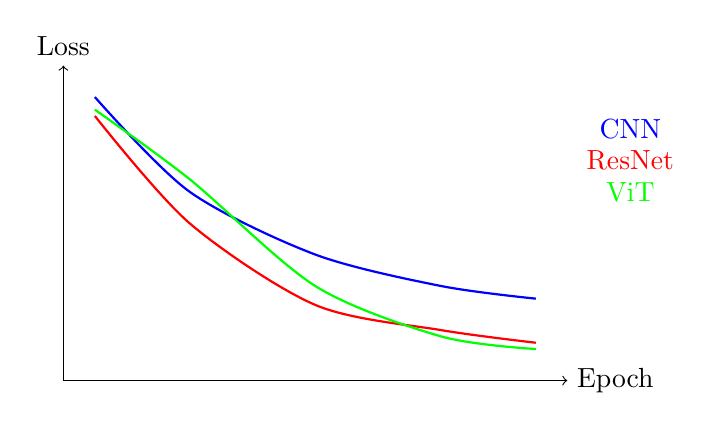
\begin{tikzpicture}[scale=0.8]
    % Axes
    \draw[->] (0,0) -- (8,0) node[right] {Epoch};
    \draw[->] (0,0) -- (0,5) node[above] {Loss};
    
    % CNN (slow convergence)
    \draw[thick, blue] plot[smooth] coordinates {(0.5,4.5) (2,3) (4,2) (6,1.5) (7.5,1.3)};
    
    % ResNet (faster, lower)
    \draw[thick, red] plot[smooth] coordinates {(0.5,4.2) (2,2.5) (4,1.2) (6,0.8) (7.5,0.6)};
    
    % ViT (starts slow, then fast)
    \draw[thick, green] plot[smooth] coordinates {(0.5,4.3) (2,3.2) (4,1.5) (6,0.7) (7.5,0.5)};
    
    % Legend
    \node[blue] at (9,4) {CNN};
    \node[red] at (9,3.5) {ResNet};
    \node[green] at (9,3) {ViT};
\end{tikzpicture}
\caption{Illustrative Training Loss Curves}
\end{figure}

\subsection{Interpretation}

\begin{tcolorbox}[colback=green!5!white,colframe=green!75!black,title=Training Dynamics]
\textbf{CNN:}
\begin{itemize}
    \item Converges slowly
    \item Higher final loss
    \item Limited capacity
\end{itemize}

\textbf{ResNet:}
\begin{itemize}
    \item Fast initial drop due to skip connections
    \item Stable convergence
    \item Good generalization
\end{itemize}

\textbf{ViT:}
\begin{itemize}
    \item Slow start (no inductive bias)
    \item Accelerates as attention learns patterns
    \item Can achieve lowest loss with enough data
\end{itemize}
\end{tcolorbox}

\section{Per-Class Analysis}

\subsection{Performance by Disease}

\begin{table}[H]
\centering
\caption{Estimated Per-Class AUC (based on paper trends)}
\begin{tabular}{lcccc}
\toprule
\textbf{Disease} & \textbf{Prevalence} & \textbf{CNN} & \textbf{ResNet} & \textbf{ViT-ResNet} \\
\midrule
No Finding & 53.84\% & 0.85 & 0.88 & 0.89 \\
Infiltration & 17.74\% & 0.78 & 0.82 & 0.84 \\
Effusion & 11.88\% & 0.80 & 0.85 & 0.86 \\
Atelectasis & 10.31\% & 0.75 & 0.80 & 0.82 \\
Nodule & 5.65\% & 0.70 & 0.78 & 0.80 \\
Pneumothorax & 4.73\% & 0.82 & 0.88 & 0.89 \\
Mass & 5.16\% & 0.72 & 0.80 & 0.82 \\
Consolidation & 4.16\% & 0.73 & 0.79 & 0.81 \\
\textcolor{red}{Hernia} & \textcolor{red}{0.20\%} & \textcolor{red}{0.65} & \textcolor{red}{0.72} & \textcolor{red}{0.75} \\
\textcolor{red}{Pneumonia} & \textcolor{red}{1.28\%} & \textcolor{red}{0.68} & \textcolor{red}{0.75} & \textcolor{red}{0.78} \\
\bottomrule
\end{tabular}
\end{table}

\subsection{Analysis}

\begin{tcolorbox}[colback=red!5!white,colframe=red!75!black,title=Class Imbalance Effect]
\textbf{Rare diseases (Hernia, Pneumonia) have lower AUC:}
\begin{itemize}
    \item Very few positive samples for training
    \item Model may not see enough examples to learn patterns
    \item High variance in predictions
\end{itemize}

\textbf{Potential Solutions:}
\begin{itemize}
    \item Class weighting in loss function
    \item Oversampling rare classes
    \item Focal loss
    \item Data augmentation specifically for rare classes
\end{itemize}
\end{tcolorbox}

\section{Computational Efficiency}

\begin{table}[H]
\centering
\caption{Computational Comparison}
\begin{tabular}{lcccc}
\toprule
\textbf{Model} & \textbf{Parameters} & \textbf{FLOPs} & \textbf{Train Time/Epoch} & \textbf{Inference Time} \\
\midrule
CNN & 102M & Low & Fast & Fast \\
ResNet-34 & 21M & Medium & Medium & Medium \\
ViT-v1/32 & ~3M & Medium & Medium & Medium \\
ViT-ResNet/16 & ~15M & High & Slow & Medium \\
\bottomrule
\end{tabular}
\end{table}

\begin{tcolorbox}[colback=blue!5!white,colframe=blue!75!black,title=Trade-offs]
\textbf{CNN:}
\begin{itemize}
    \item Most parameters but fastest (simple operations)
    \item Good for edge deployment
\end{itemize}

\textbf{ViT:}
\begin{itemize}
    \item Self-attention is $O(n^2)$ in sequence length
    \item 49 patches → 49² = 2401 attention computations per head
    \item Scales poorly with image resolution
\end{itemize}

\textbf{ViT-ResNet:}
\begin{itemize}
    \item More patches (196) but smaller embedding
    \item Best accuracy/computation trade-off
\end{itemize}
\end{tcolorbox}

\section{Discussion}

\paperref{Section 6 - Discussion}

\subsection{Key Findings}

\begin{tcolorbox}[colback=yellow!5!white,colframe=yellow!75!black,title=Paper Discussion Quote]
\textit{``Our experiments revealed that using a deeper, more complex model architecture leads to better diagnostic accuracy. We trained 5 models: a baseline CNN, a ResNet, and 3 different versions of Vision Transformers. We observe that the best-performing model architecture is ViT-ResNet, which combines features of ResNets as well as Vision Transformers.''}
\end{tcolorbox}

\subsection{Limitations}

\begin{tcolorbox}[colback=red!5!white,colframe=red!75!black,title=Limitations Identified]
\begin{enumerate}
    \item \textbf{Weak Labels:}
    \begin{itemize}
        \item NIH labels extracted via NLP from reports
        \item May contain noise and errors
        \item Not radiologist-verified ground truth
    \end{itemize}
    
    \item \textbf{Class Imbalance:}
    \begin{itemize}
        \item Severe imbalance (Hernia: 0.2\%)
        \item Models may be biased toward common classes
    \end{itemize}
    
    \item \textbf{Multi-label Complexity:}
    \begin{itemize}
        \item Patients can have multiple conditions
        \item Label co-occurrence patterns may confuse model
    \end{itemize}
    
    \item \textbf{Data Split:}
    \begin{itemize}
        \item No mention of patient-level split
        \item Potential data leakage risk
    \end{itemize}
\end{enumerate}
\end{tcolorbox}

\section{Conclusion from Experiments}

\begin{tcolorbox}[colback=green!5!white,colframe=green!75!black,title=Experimental Conclusions]
\begin{enumerate}
    \item \textbf{Architecture matters:} Deeper and more sophisticated architectures (ResNet, ViT) outperform simple CNN
    
    \item \textbf{Hybrid is best:} ViT-ResNet combines:
    \begin{itemize}
        \item CNN's local feature extraction
        \item Transformer's global reasoning
    \end{itemize}
    
    \item \textbf{Skip connections are crucial:} ResNet's 2\% improvement over CNN shows importance of residual learning
    
    \item \textbf{Transformers need care:} Pure ViT comparable to ResNet but requires more tuning
    
    \item \textbf{All models viable:} Even CNN (91\%) could be useful in resource-constrained settings
\end{enumerate}
\end{tcolorbox}
